\documentclass{article}
\usepackage{amsmath}
\usepackage{graphicx}
\usepackage[hidelinks]{hyperref}

\begin{document}
    
\title{Game Theory of Hoot Owl Hoot}
\author{Mike Blemberg}
\maketitle

\begin{abstract}
A game theory analysis of the board game Hoot Owl Hoot.  A probabilistic analysis of lost games is calculated for games played with two, three, or four players.  
\end{abstract}

\section{Rules of the Game}
The rules of Hoot Owl Hoot are summarized here for convenience and the official rules can be found on the website of the manufacturer, Mindware, at the following link.

\url{https://s7.orientaltrading.com/is/content/OrientalTrading/PDFs/HootOwlHoot_Instructions.pdf}

\subsection{Equipment}

\subsection{Board}

\subsection{Turns}

\subsection{Objective}


\section{How a Game is Lost}
In Hoot Owl Hoot, a game is lost when the sun token reaches the final sun space.  This occurs when 13 sun cards have been played and the sun token has been moved 13 times.

\section{Position of the 13th Sun Card}
The probability that the 13th sun card exists at a specific position, $k$, in the deck is calculated using the following information.

\begin{enumerate}
    \item There are a total of 14 sun cards distributed throughout the 50 card deck.
    \item 12 sun cards are distributed in the cards before the 13th sun card.
    \item One sun card is positioned somewhere in the deck after the 13th sun card.
\end{enumerate}

The number of possible ways to distribute 14 suns in a 50 card deck is calculated using a binomial coefficient as shown in Equation \ref{eq:total_combinations}.

\begin{equation} \label{eq:total_combinations}
  N_{deck\_combination} = \binom{50}{14}
\end{equation}

The number of possible ways to distribute 12 sun cards before the $kth$ position is calculated similarly in Equation \ref{eq:12_suns_combinations}.

\begin{equation} \label{eq:12_suns_combinations}
  N_{12\_sun\_combinations} = \binom{k-1}{12}
\end{equation}

And the number of possible locations for the 14th sun card is simply $50-k$.  As a result, the probability that the 13th sun card is located at position $k$ is calculated in Equation \ref{eq:pdf_13th_sun}.

\begin{equation} \label{eq:pdf_13th_sun}
  p(k) = \frac{\binom{k-1}{12} \left( 50-k \right)}{\binom{50}{14}}
\end{equation}



The resulting probability distribution function is shown in Figure \ref{fig:13th_sun_pdf}.

\begin{figure}
  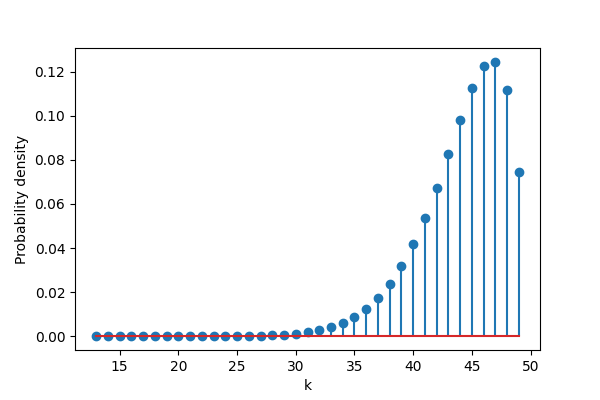
\includegraphics[width=\linewidth]{pdf_13th_sun_position.png}
  \caption{Probability density function for the position, $k$, of the 13th sun card within the deck.}
  \label{fig:13th_sun_pdf}
\end{figure}

The expected position of the 13th sun, $E[k_{13}]$, is calculated in Equation \ref{eq:expected_position_13th_sun}.

\begin{equation} \label{eq:expected_position_13th_sun}
\begin{split}
E[k_{13}] & = \sum_{k=13}^{49}p(k)k \\
& = \sum_{k=13}^{49} \left[ \frac{\binom{k-1}{12} \left( 50-k \right)k}{\binom{50}{14}} \right] \\
& = \sum_{k=13}^{49} \left[ \frac{(k-1)!(50k-k^{2})} {(k-13)!} \frac{14!*36!}{12!*50!} \right] \\
& = 44.2
\end{split}
\end{equation}

\section{Average Number of Cards Played in a Lost Game}
Since a player must play a sun card if they have one, the number of cards played in a lost game is directly related to the position of the 13th sun card in the deck.  Each player begins the game with two cards that they don't play on their first turn, so the number of cards played is calculated in Equation \ref{eq:avg_cards_played}.  The average numbers of cards played in games with different numbers of players are listed in Table \ref{tb:avg_cards_played}.

\begin{equation} \label{eq:avg_cards_played}
  E[N_{cards\_played}] = E[k_{13}] - 2 N_{players}
\end{equation}

\begin{table}
  \centering
  \begin{tabular}{| c | c |}
    \hline
    Number of Players & Avg. Cards Played \\ \hline
    2 & 42.2 \\ \hline
    3 & 40.2 \\ \hline
    4 & 38.2 \\ \hline
  \end{tabular}
  \caption{The average number of cards played in games with different numbers of players.}
  \label{tb:avg_cards_played}
  \end{table}


\end{document}